\documentclass{article}
\usepackage[utf8]{inputenc}
\usepackage{enumerate}
\usepackage{mathtools}
\usepackage{hyperref}
\usepackage{pdfpages}
\usepackage{caption}
\usepackage{titling}
\usepackage{pgfplots}
\usepgfplotslibrary[fillbetween]
\usetikzlibrary[patterns]
\usepackage{amsmath}
\usepackage{geometry}
\usepackage{subcaption}
\usepackage{graphicx}
\usepackage{stfloats}

\setlength{\droptitle}{-10em}

\author{Magnus Moan}
\title{IT3708: Project 4}
\geometry{
  bottom=2cm
}

\begin{document}


\maketitle

\section*{Task 1}
\subsection*{Particle Swarm Optimization and Bees Algorithm}
I use the same representation for my Particle Swam Optimization (PSO) and Bees Algorithm (BA). The representation is an indirect representation. Each individual (particle in PSO and bee in BA) is represented as a one dimensional array of length equal
to the number of operations ($nOperations$) to be scheduled in the problem. The number of operations is equal to the number of jobs multiplied with the number of machines:
\begin{equation*}
  nOperations = nJobs\,\times\,nMachines
\end{equation*}
The values in the array are floating point numbers in the range $[0, nOperations]$. The floating point numbers are randomly initialized. This representation is usually refered to as a vector in RK space in the literature. To go from this representation to a feasible schedule I perform the following steps:
\begin{enumerate}
  \item Go from the continuous space to a discrete space by creating a new array with integers in the range $[0, nOperations]$. Sort these integers according to the rank of the floating point numbers. See Figure \ref{fig:repr} for example (line with "an integer series").
  \item Transform the integer array to another integer array representing the different jobs by taking the modulus of the integer number in each position of the vector. See Figure \ref{fig:repr} for example. The resulting vector will consist of $nJobs$ unique numbers which are
    repeated exactly $nMachines$ times.
  \item A feasible schedule can be created from this representation. This is done by traversing the vector of jobs and for each integer (which represents a job) do the following:
    \begin{enumerate}[i)]
      \item Find the next machine this specific job needs to prosseced by. 
      \item Check the next available time for this specific job (it might by occupied by some other machine) as well as the next available job for the machine needed (the machine might be occupied by another job)
      \item Set the starting time of the current job at the current machine equal to the maximum of the two times found in step ii).
      \item Update the next available time for both the machine and the job.
    \end{enumerate}
\end{enumerate}

\begin{figure}[h!]
  \centering
  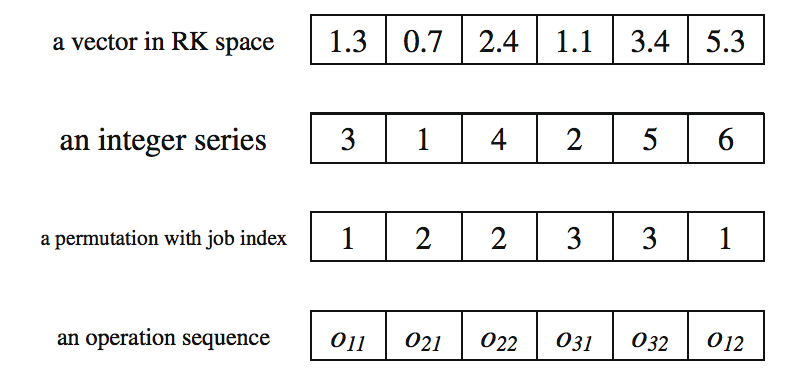
\includegraphics[scale=.4]{repr.png}
  \caption{The different steps from individual representation to operation sequence}
  \label{fig:repr}
\end{figure}

\pagebreak
\subsubsection*{Ant Colony Optimization}
For the Ant Colony Optimization (ACO) I use a direct representation. Each ant have an array consisting of tuples. Each tuple represents an operation. An operation consist of a job number, a machine number and a duration.
My algorithm create this array in an iterative fashion for each ant in each iteration. During the creation of the array I make sure that it's only to add operations that keeps the resulting schedule feasible. This is done by always picking between
operations where all precessor operations have alredy been added to the array. A precessor operation is an operation that is earlier than the current operation in same jobs technological sequence. When I first have this array I already know that it's
feasible. Creating a schedule from it is straight forward. This can be done by iterating over the array in the same fashion as in steps ii)-iv) above. Step i) is not neseccary since I in this representation already know the machine. See Table \ref{ant} for an 
example of an array with operations.

\begin{table}[h!]
  \centering
  \caption{Ant representation w/ corresponding problem instance}
  \subcaption*{Ant representation}
\begin{tabular}{|l|l|l|l|l|l|}
\hline
(2,1,1) & (2,0,1) & (1,1,3) & (0,0,2) & (1,0,1) & (1,0,1) \\ \hline
\end{tabular} \\[2ex]
\subcaption*{Problem instance. m = machine, t = time}
\begin{tabular}{|l|c|c|}
  \hline
Job-n & \multicolumn{1}{l|}{(m, t)} & \multicolumn{1}{l|}{(m, t)} \\ \hline
Job-0 & (0,2)                               & (1,2)                               \\ \hline
Job-1 & (1,3)                               & (0,1)                               \\ \hline
Job-2 & (1,1)                               & (0,1)                               \\ \hline
\end{tabular}
\label{ant}
\end{table}
\pagebreak
\section*{Task 2}
\begin{figure}[h]
  \centering
  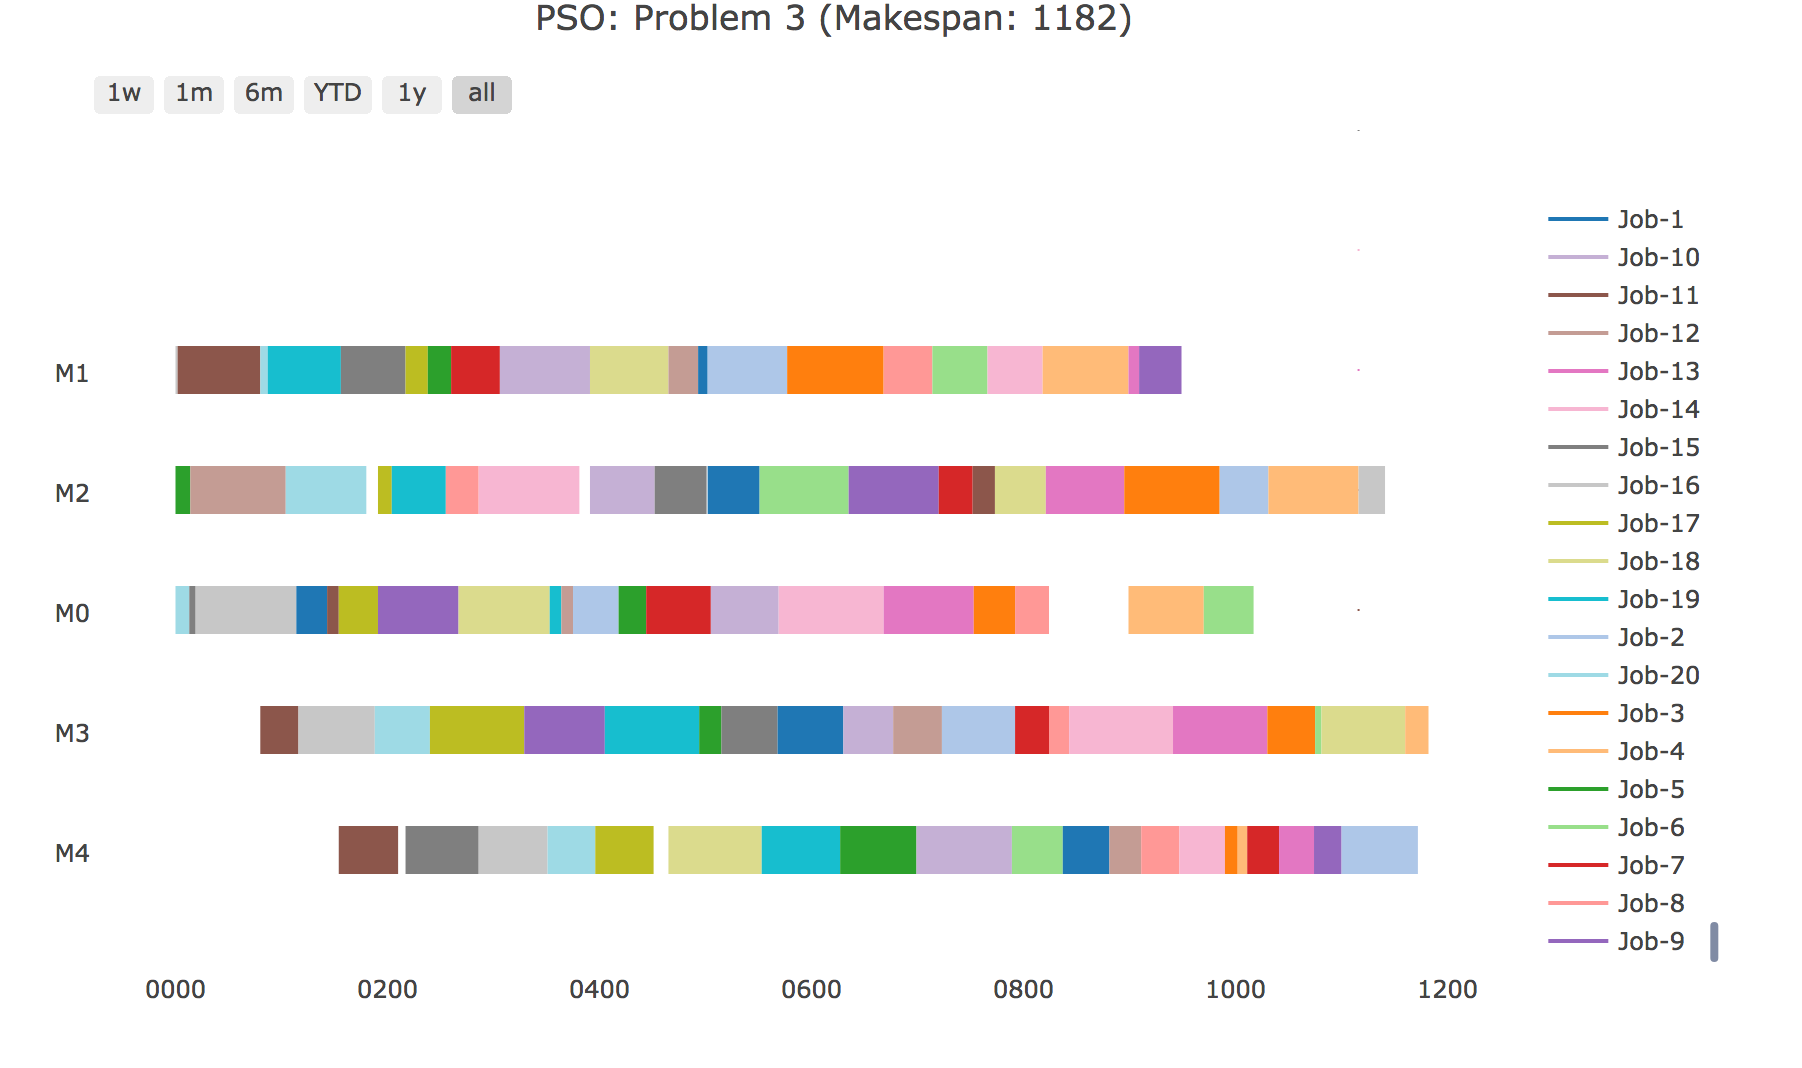
\includegraphics[scale=.45]{../Results/PNG/pso_3.png}
\end{figure}
\vspace{-1cm}
\begin{figure}[h!]
  \centering
  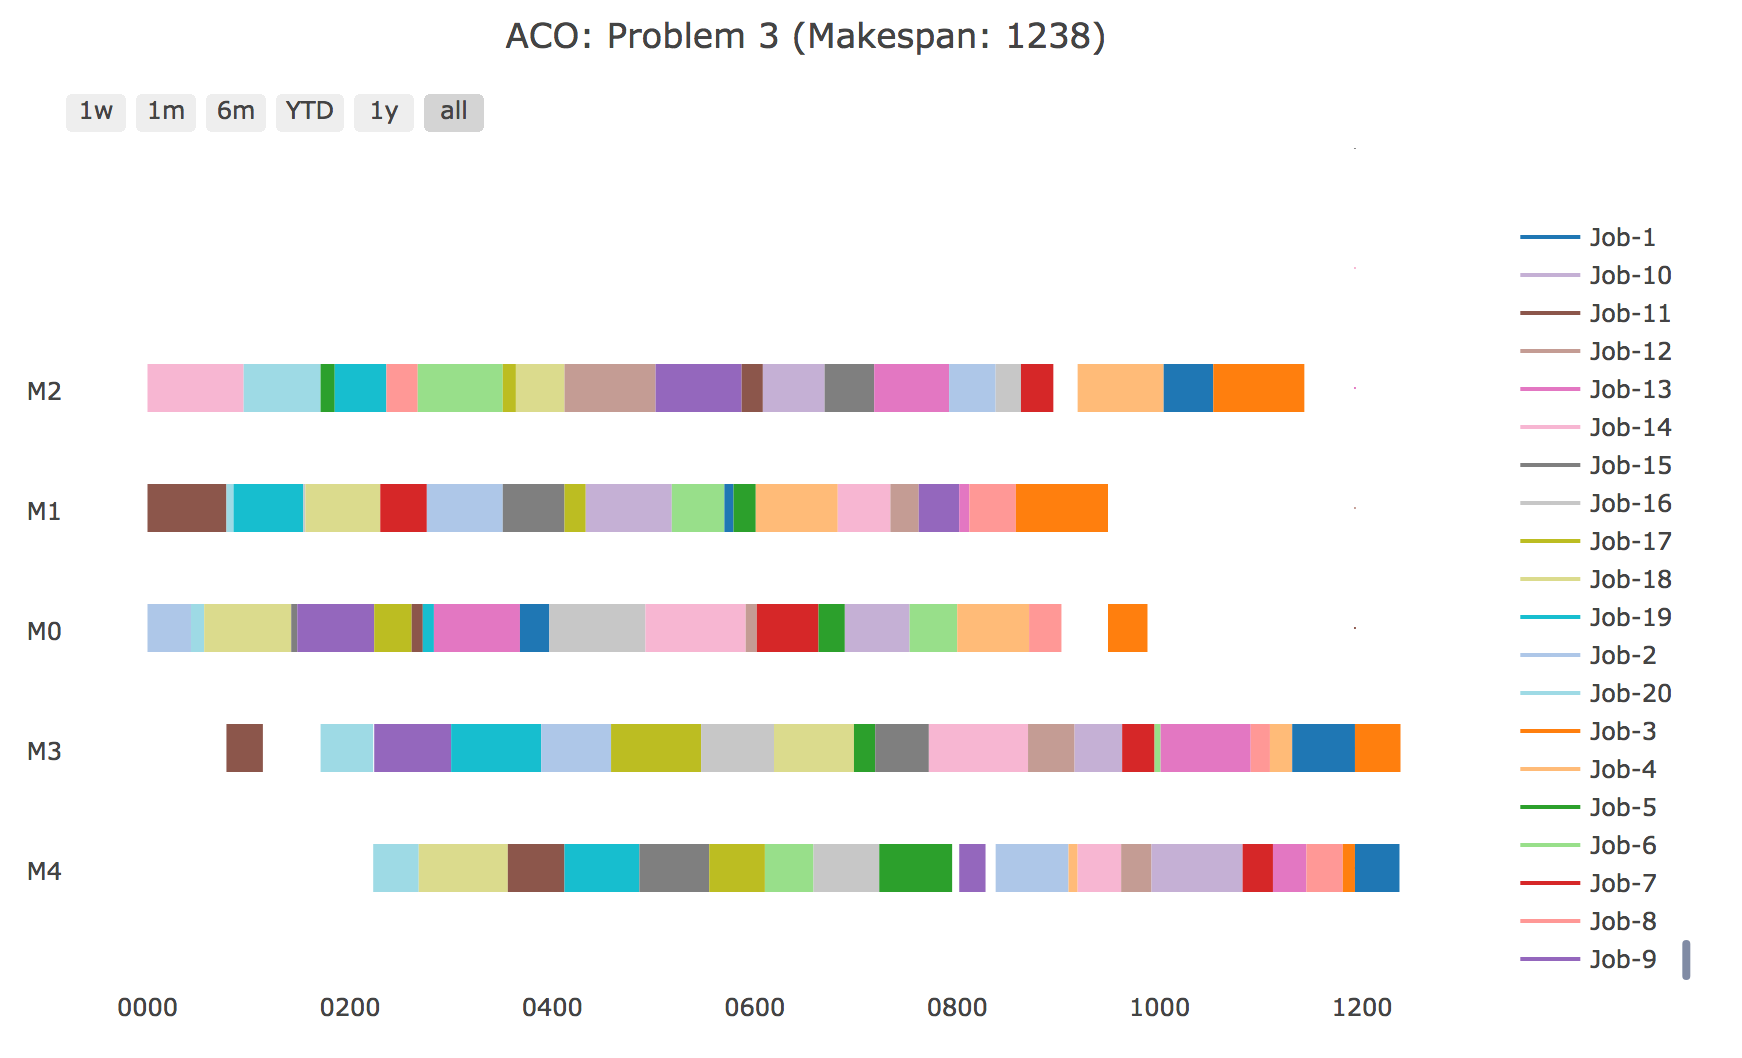
\includegraphics[scale=.45]{../Results/PNG/aco_3.png}
\end{figure}

\begin{figure}[h]
  \centering
  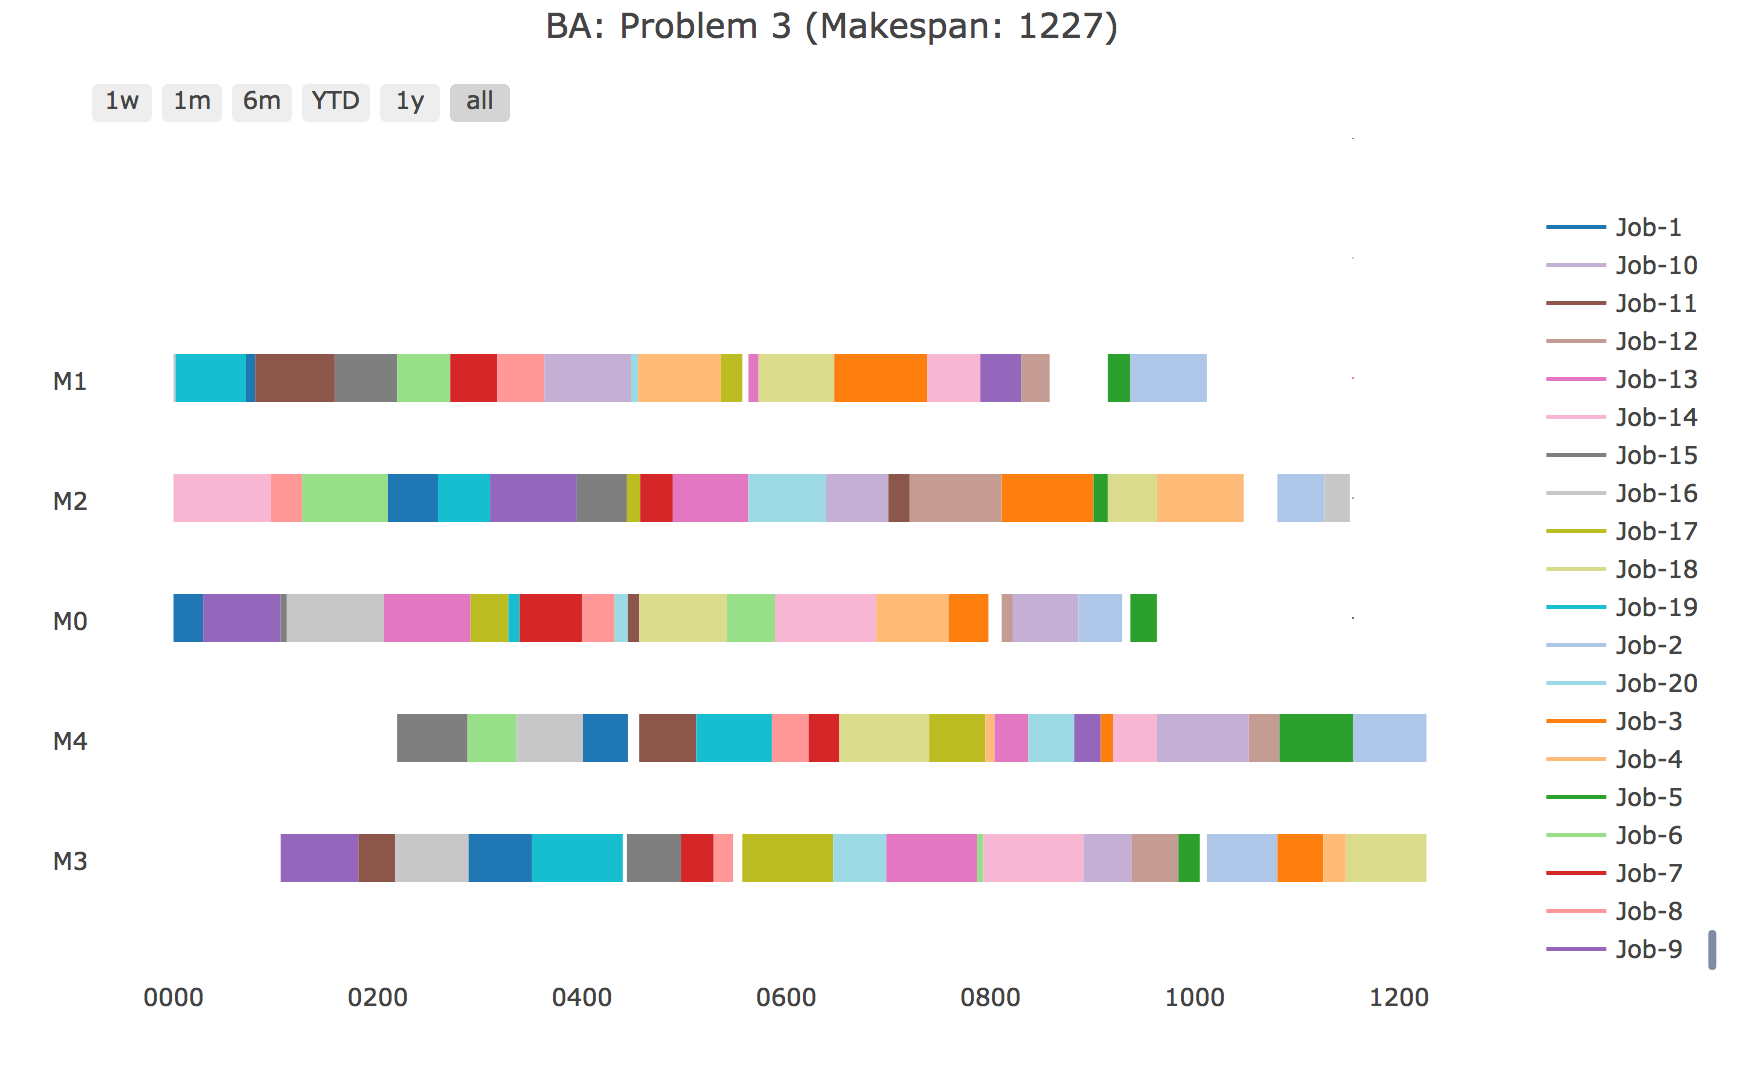
\includegraphics[scale=.45]{../Results/PNG/ba_3.png}
\end{figure}
\end{document}
